\hypertarget{elliptic-curve-cryptography}{%
\section{Elliptic Curve
Cryptography}\label{elliptic-curve-cryptography}}

Warum? Die Elliptischen Kurven sind performanter!

\hypertarget{definition}{%
\subsection{Definition}\label{definition}}

Weierstrass equation for an elliptic curve

\begin{figure}[H]
\centering
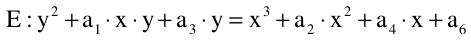
\includegraphics[width=0.4\textwidth]{figures/weierstrasseEquation.png}
\caption{Weierstrass Equation}
\end{figure}

\begin{itemize}
\tightlist
\item
  The set of points $(x,y)$ that satisfy this equation is an elliptic
  curve.
\item
  The coefficients $a_i$ can be elements of any field F.
\item
  The strange numbering of the coefficients is an artifact of the
  process by which the above equation was derived.
\item
  The points of the elliptic curve, together with an extra point O,
  called the point at infinity, can be uses to define an additive group
\end{itemize}

\hypertarget{vereinfachung}{%
\subsection{Vereinfachung}\label{vereinfachung}}

When the field $F$ over which the elliptic curve is defined has
characteristic other than 2 or 3 the Weierstrass equation can be
simplified.

\begin{tcolorbox}[colback=red!5!white,colframe=red!75!black]
    $y^2 = x^3 + a * x + b$
    
    An elliptic curve that is defined by this equation can be used to form a group if \\
    $4 * a^3 + 27 * b^2 \neq 0$ and $x^3 + a * x + b$ containts no multiple roots  \\
    $\Rightarrow$ These two conditions are equivalent
\end{tcolorbox}

\begin{figure}[H]
\centering
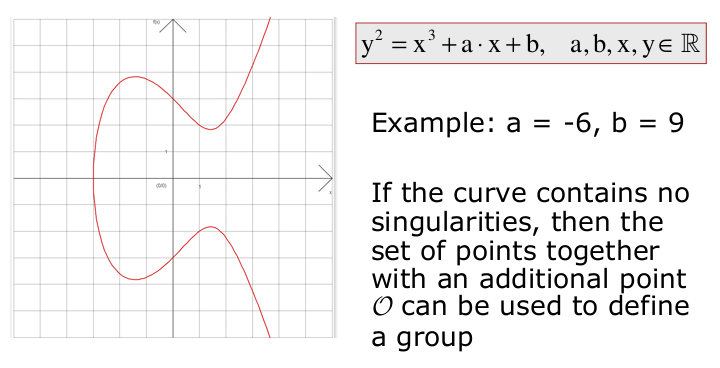
\includegraphics[width=0.7\textwidth]{figures/ellipticCurveRealNumbers.png}
\caption{Elliptic Curve of the Real Numbers}
\end{figure}

\hypertarget{addition-of-different-points}{%
\subsection{Addition of different
Points}\label{addition-of-different-points}}

\begin{figure}[H]
\centering
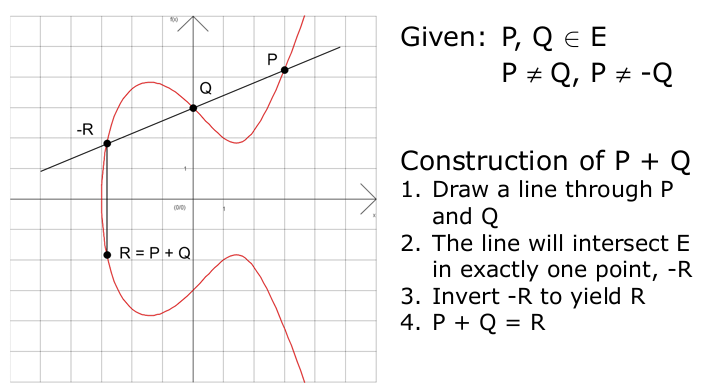
\includegraphics[width=0.7\textwidth]{figures/additionEllipse.png}
\caption{Elliptic Curve - Addition of different Points}
\end{figure}

Man nimmt ein Lineal und zeichnet eine Gerade durch $P$ und $Q$. Dort wo die Gerade die Ellipsische
Kurve wieder schneidet ($-R$), mache ich noch einmal eine Gerade durch
diesen Punkt ($-R$) im 90° Winkel zur X-Achse und das ergibt $R$, was das
Resultat von $Q+P$ ist.

\hypertarget{addition-of-p-and--p}{%
\subsection{Addition of P and -P}\label{addition-of-p-and--p}}

\begin{figure}[H]
\centering
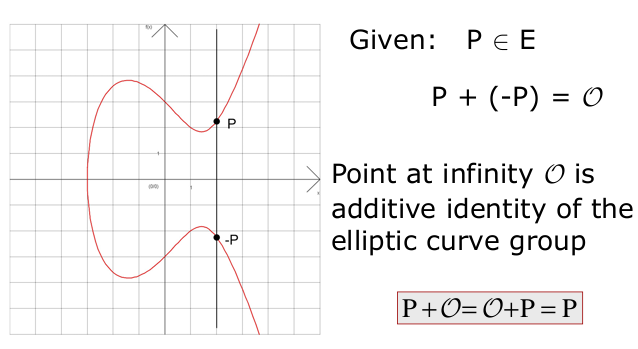
\includegraphics[width=0.7\textwidth]{figures/addition2Ellipse.png}
\caption{Elliptic Curve - Addition of inverse Points}
\end{figure}

Falls die Punkte $P$ und $-P$ addiert werden müssen, schneidet die Gerade dieser beiden Punkte die
elliptische Kurve nicht mehr. ABER diese Gerade schneidet die elliptische Kurve im Unendlichen.

\begin{tcolorbox}[colback=red!5!white,colframe=red!75!black]
Der Punkt im Unendlichen ist das neutrale Element jeden Körpers.
Irgendein Punkt P + der Punkt im Unendlichen ergibt den Punkt P.
\end{tcolorbox}

\hypertarget{doubling-p}{%
\subsection{Doubling P}\label{doubling-p}}

\begin{figure}[H]
\centering
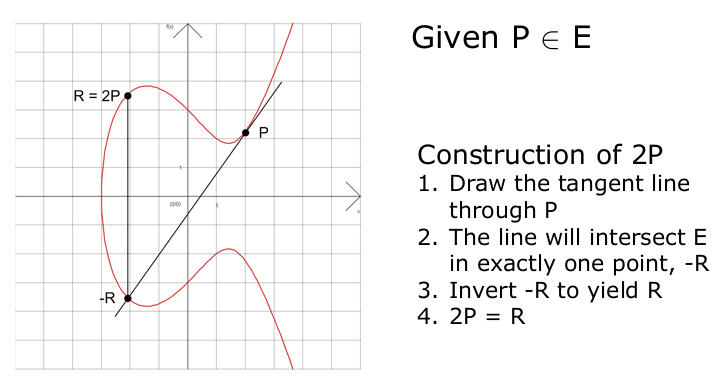
\includegraphics[width=0.7\textwidth]{figures/doublePellipse.png}
\caption{Elliptic Curve - Doubling of two Points}
\end{figure}

Um den Punkt P zu verdoppeln, muss ich die Tangente an den Punkt P legen. Danach die
gleichen Schritte machen wie beim Addieren.

\hypertarget{algebraische-luxf6sung}{%
\subsection{Algebraische Lösung}\label{algebraische-luxf6sung}}

\begin{figure}[H]
\centering
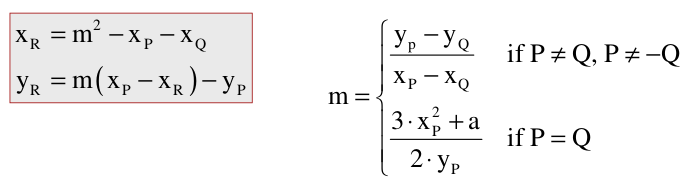
\includegraphics[width=0.5\textwidth]{figures/algebraicSolutionEllipse.png}
\caption{Formeln algebraische Lösung}
\end{figure}

Die Berechnung der Steigung sieht ein wenig anders aus, falls $P = Q$ ist.

Spezialfälle ($O$ ist Punkt im Unendlichen):\\
$O + O = O$\\
$P + O = O + P = P$\\
$P + ( - P) = O$

\hypertarget{elliptic-curve-over-gf23}{%
\subsection{Elliptic Curve over GF(23)}\label{elliptic-curve-over-gf23}}

\begin{figure}[H]
\centering
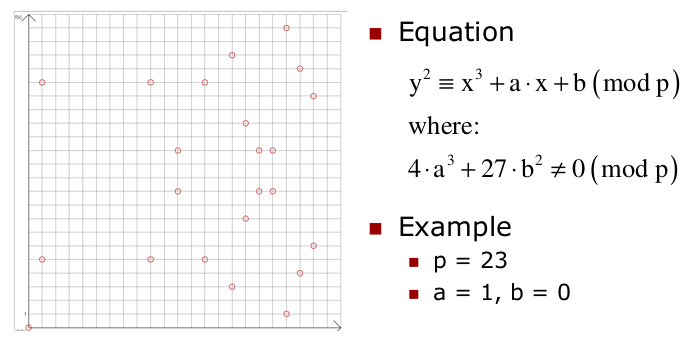
\includegraphics[width=0.7\textwidth]{figures/ellipticCurveGf23.png}
\caption{Elliptic Curve over GF(23)}
\end{figure}

\begin{itemize}
\tightlist
\item
  Das heisst auch das Koordinatensystem hat maximale Werte bis 23.
\item
  Nun kann man dieselben Formen benutzen, wie wir sie vorher berechnet
  haben.
\item
  Für Addition und Divison kann man nun die Operationen des endlichen
  Körpers anwenden.
\end{itemize}

\hypertarget{theorem-of-hasse}{%
\subsubsection{Theorem of Hasse}\label{theorem-of-hasse}}

Wenn wir die Anzahl Punkte der elliptischen Kurve im Körper GF(p) berechnen, inklusive der Punkt im Unendlichen, gilt folgendes:

\begin{figure}[H]
\centering
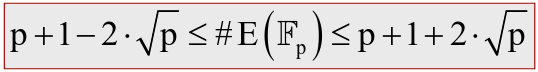
\includegraphics[width=0.5\textwidth]{figures/theoremHasse.png}
\caption{Theorem of Hasse}
\end{figure}

\hypertarget{adding-distinct-points}{%
\subsubsection{Adding distinct points}\label{adding-distinct-points}}

Eigentlich sind das nun dieselben Formen, jedoch muss beachtet werden
dass nun keine Divisonen mehr erlaubt sind.

\begin{figure}[H]
\centering
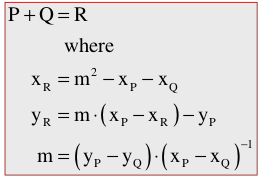
\includegraphics[width=0.3\textwidth]{figures/addingDistinctPointsoverGF.png}
\caption{Adding distinct Points over GF}
\end{figure}

\clearpage
\hypertarget{doubling-a-point}{%
\subsubsection{Doubling a point}\label{doubling-a-point}}

Auch hier, keine Division
\begin{figure}[H]
\centering
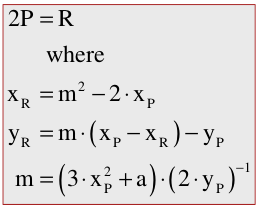
\includegraphics[width=0.3\textwidth]{figures/doublingPointOverGf.png}
\caption{Division of two distinct Points over GF}
\end{figure}

\hypertarget{order-of-a-point}{%
\subsection{Order of a Point}\label{order-of-a-point}}

Durch fortlaufende Addition des Punktes $P$ kann ich auch $n*P$ berechnen.

Die Ordnung von $G$ bedeutet: Wie lange kann ich $G$ mit sich selbst
addieren, bis ich den Punkt im Unendlichen bekomme? $\Rightarrow$ Die kleinste
nicht-negative Ganzzahl ist die Ordnung von $G$.

Wenn ich alle Elemente innerhalb des Körpers nehme und durch die Ordnung
$n$ teile, ergibt das immer eine Ganzzahl. (nennt man auch manchman
Co-Faktor)

\begin{tcolorbox}[colback=red!5!white,colframe=red!75!black]
Der Punkt im Unendlichen hat immer die Ordnung 1.
\end{tcolorbox}

\hypertarget{elliptic-curve-domain-parameters}{%
\subsection{Elliptic Curve Domain
Parameters}\label{elliptic-curve-domain-parameters}}

Folgende Parameter sind im Standard definiert:

\begin{figure}[H]
\centering
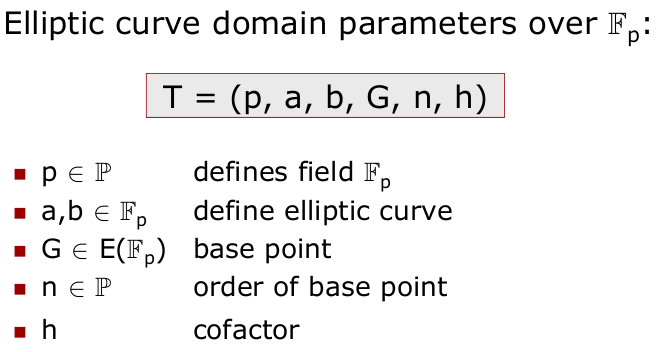
\includegraphics[width=0.5\textwidth]{figures/ellipticCurveDomainParameters.png}
\caption{Elliptic Curve Domain Parameters}
\end{figure}

\hypertarget{elliptic-curve-diffie-hellman-ecdh}{%
\subsection{Elliptic curve Diffie-Hellman
(ECDH)}\label{elliptic-curve-diffie-hellman-ecdh}}

\begin{figure}[H]
\centering
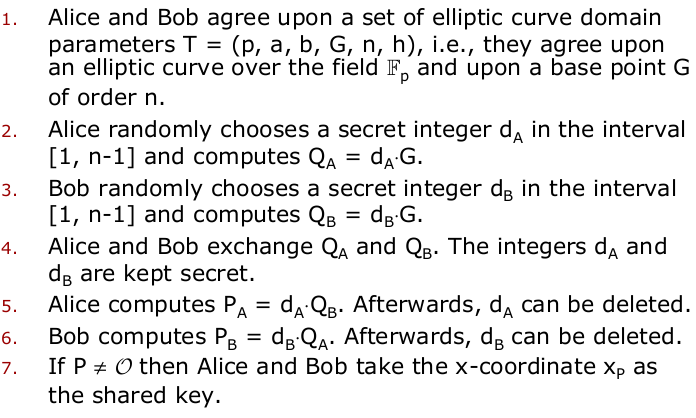
\includegraphics[width=0.75\textwidth]{figures/ecdh.png}
\caption{ECDH}
\end{figure}

\begin{figure}[H]
\centering
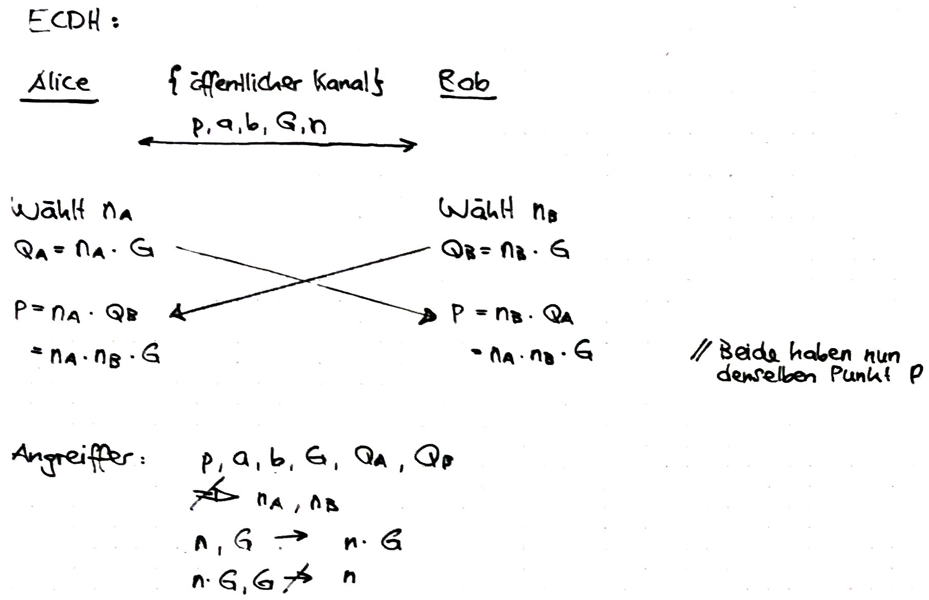
\includegraphics[width=0.75\textwidth]{figures/notesEcdh.png}
\caption{Notes ECDH}
\end{figure}

\hypertarget{elliptic-curve-discrete-logarithm-problem}{%
\subsection{Elliptic Curve Discrete Logarithm Problem}\label{elliptic-curve-discrete-logarithm-problem}}

The ECDLP is believed to be hard to solve, even with today's
computational power!. $\Rightarrow$ Bedeutet in diesem Fall, dass man vermutlich einfach alles durchprobieren muss (Bruteforce!)

\hypertarget{weitere-funktionen}{%
\subsection{Weitere Funktionen}\label{weitere-funktionen}}

Es ist mit elliptischen Kurven auch möglich, Nachrichten zu verschlüsseln oder zu unterschreiben. Auf dies gehen wir jedoch nicht stark ein.

\clearpage
